\documentclass[11pt]{article}
\usepackage[margin=1in]{geometry}
\usepackage{amsmath,amssymb,amsthm}
\usepackage{graphicx}
\usepackage{float}
\usepackage[onehalfspacing]{setspace}
\usepackage[unicode=true,
 bookmarks=true,bookmarksnumbered=false,bookmarksopen=false,
 breaklinks=false,pdfborder={0 0 0},pdfborderstyle={},backref=false,colorlinks=true]
 {hyperref}
\usepackage{verbatim}
\usepackage{appendix}
\usepackage{mathtools}
\usepackage{url}
\usepackage[authoryear]{natbib}
\usepackage{soul}
\usepackage{tikz}
\usetikzlibrary{calc}
\usepackage{caption}
\usepackage{subcaption}
\usepackage{comment}
\usepackage{ulem}
\usepackage{setspace}
\usepackage[en-US]{datetime2}

\renewcommand{\v}[1]{\ensuremath{\mathbf{#1}}} % for vectors
\newcommand{\gv}[1]{\ensuremath{\mbox{\boldmath$ #1 $}}} 
% for vectors of Greek letters
\newcommand{\uv}[1]{\ensuremath{\mathbf{\hat{#1}}}} % for unit vector
\newcommand{\abs}[1]{\left| #1 \right|} % for absolute value
\newcommand{\avg}[1]{\left< #1 \right>} % for average
\let\underdot=\d % rename builtin command \d{} to \underdot{}
\renewcommand{\d}[2]{\frac{d #1}{d #2}} % for derivatives
\newcommand{\dd}[2]{\frac{d^2 #1}{d #2^2}} % for double derivatives
\newcommand{\pd}[2]{\frac{\partial #1}{\partial #2}} 
% for partial derivatives
\newcommand{\pdd}[2]{\frac{\partial^2 #1}{\partial #2^2}} 
% for double partial derivatives
\newcommand{\pdc}[3]{\left( \frac{\partial #1}{\partial #2}
 \right)_{#3}} % for thermodynamic partial derivatives
\newcommand{\ket}[1]{\left| #1 \right>} % for Dirac bras
\newcommand{\bra}[1]{\left< #1 \right|} % for Dirac kets
\newcommand{\braket}[2]{\left< #1 \vphantom{#2} \right|
 \left. #2 \vphantom{#1} \right>} % for Dirac brackets
\newcommand{\matrixel}[3]{\left< #1 \vphantom{#2#3} \right|
 #2 \left| #3 \vphantom{#1#2} \right>} % for Dirac matrix elements
\newcommand{\grad}[1]{\gv{\nabla} #1} % for gradient
\let\divsymb=\div % rename builtin command \div to \divsymb
\renewcommand{\div}[1]{\gv{\nabla} \cdot \v{#1}} % for divergence
\newcommand{\curl}[1]{\gv{\nabla} \times \v{#1}} % for curl
\newcommand{\stkout}[1]{\ifmmode\text{\sout{\ensuremath{#1}}}\else\sout{#1}\fi}
\newcommand{\msout}[1]{\text{\sout{\ensuremath{#1}}}}
\let\baraccent=\= % rename builtin command \= to \baraccent
\renewcommand{\=}[1]{\stackrel{#1}{=}} % for putting numbers above =
\providecommand{\wave}[1]{\v{\tilde{#1}}}
\providecommand{\fr}{\frac}
\providecommand{\RR}{\mathbb{R}}
\providecommand{\NN}{\mathbb{N}}
\providecommand{\seq}{\subseteq}
\providecommand{\e}{\epsilon}
\newtheorem{prop}{Proposition}
\newtheorem*{lem}{Lemma}
\theoremstyle{definition}
\newtheorem*{dfn}{Definition}
\newenvironment{s}{%\small%
        \begin{trivlist} \item \textbf{Solution}. }{%
            \hspace*{\fill} $\blacksquare$\end{trivlist}}%
\newenvironment{p}{}{}
\DeclareMathOperator*{\argmax}{arg\,max}
\DeclareMathOperator*{\argmin}{arg\,min}

\hypersetup{
	pdftex,
    pdfauthor={Jonathan I. Dingel and friends},     % author
    colorlinks=true,       % false: boxed links; true: colored links
    linkcolor=red,          % color of internal links
    citecolor=black,        % color of links to bibliography
    urlcolor=blue           % color of external links
}

% CUSTOM DEFINITIONS
\urldef{\dingelhomepage}\url{http://faculty.chicagobooth.edu/jonathan.dingel/}
\urldef{\rufemail}\url{jcruf@uchicago.edu}
\newtheorem{proposition}{Proposition}

% IDENTIFYING INFORMATION
\title{How does Experience effect Politicians' Spending Priorities? Evidence from Chicago's Aldermanic Menu Program}
\author{John C. Ruf \thanks{\rufemail}}
\date{\today}


\begin{document}
\bibliographystyle{../bib/aeanobold}
\maketitle
% -----------------------------------------------
% 	ABSTRACT
% -----------------------------------------------

\begin{abstract}
\begin{spacing}{1.0}
This paper investigates the political economy of conspicuous public spending. 
It defines conspicuous public spending as spending intended to signal competency to voters for electoral gain. 
A simple career-concerns model featuring a tradeoff between conspicuous and inconspicuous expenditures with experience gain demonstrates this effect in a rational-choice framework. 
The model has two critical implications. 
Firstly, unexpected increases in conspicuous expenditures help politicians get re-elected. 
Secondly, less-experienced politicians spend more conspicuously than their established counterparts. 
This paper uses data from Chicago's Aldermanic Menu Program to test these implications. 
The first implication is confirmed via a simple discrete-choice analysis. Differences-in-differences methods further show some evidence for the second implication. 
However, counter to the model, the Differences-in-Differences study shows an effect that decays before the next election.
Furthermore, a regression discontinuity analysis also shows an increase in spending, which is not consistent with the model.
This paper concludes by exploring alternative hypotheses that may be driving the decaying effect.
\end{spacing}
\end{abstract}
\vspace{1cm}
{\small
\noindent \textit{Keywords}: Menu Program, Aldermen, Infrastructure Maintenance \\
\textit{JEL codes}: L98 H72 
}
\thispagestyle{empty}
\newpage
\setcounter{page}{1}

% -----------------------------------------------
% 	BODY
% -----------------------------------------------

%\section{Introduction}

\begin{frame}{Motivation}
    How do local politicians allocate infrastructure maintenance and other key public goods?
    \begin{itemize}
        \item (Glaeser 2019) find a strong shortage of road maintenance in the country: is it a political economy problem?
        \item If local politicians cannot be trusted to maintain key infrastructure and roads, that has important welfare implications for optimal placement of ``large'' welfare enhancing projects.
        \item How prevalent would clientelism be if we allocated public resources in a more decentralized manner?
        \item What are the costs of giving local politicians unilateral control over infrastructure maintenance? What magnitude would the benefits like ``local knowledge'' and ``accountability'' need to be to justify this?
    \end{itemize}
\end{frame}
    
\begin{frame}{What do aldermen do?}
    \begin{center}
    \begin{quotation}
        ``I remember crossing California going west, every street was resurfaced almost every year. They always had brand new lighting and then east of California, where Ald. Bernie Stone would lose the precincts consistently, I mean the streets were in shambles.'' \\
    \end{quotation}
    \end{center}
    \raggedleft{ -Ald. Carlos Ramirez-Rosa (35th Ward).}
    \begin{itemize}
        \item Aldermen as Mini-Mayor over Ward
        \begin{itemize}
            \item City council defers to Ward Alderman all internal issues
            \item Eg. \ snow plows, garbage cleanup, sign permits, business licenses, liquor-moratoriums, and of course, construction and zoning.
            \item A relatively new power that aldermen were granted in 1995 is the ability to allocate \$1.5M in infrastructure ``menu'' requests 
        \end{itemize}
    \end{itemize}
\end{frame}
    
\begin{frame}{What is the Aldermanic Menu Program?}
        Alderman have the power to allocate \$ 1.5M on a variety of infrastructure projects. They are given a map of 311 complaints for guidance.
    \begin{itemize}
        \item  5 primary categories:
        \begin{itemize}
            \item \textbf{Streets/CDOT:} Alley/Road/Sidewalk Resurfacing, speed bump replacement, sign installation, Curb and Gutter fixes, etc. 
            \item \textbf{Crime Prevention and Lighting:} Camera installation and street lights
            \item \textbf{Arts:} Murals and Neighborhood Arts programs
            \item \textbf{Schools:} Direct grants to CPS, Sports Fields, Gardens, Auditoriums, Playgrounds, etc. 
            \item \textbf{Parks, Trees, and Gardens:} Tree planting, public garden formation, and park cleanup programs. 
        \end{itemize}
    \end{itemize}
\end{frame}

\begin{frame}{2017 OIG Audit}
        The office of the inspector general (OIG) conducted an audit of the menu program in 2017.
        The audit was scathing. 
        They recommended dismantling the program and reallocating the funds to a more traditional central planning model.
        The primary findings of the audit are given below.
    \begin{enumerate}
        \item  Menu, which serves as the City's primary residential infrastructure
        program, underfunds residential infrastructure needs and results in
        significant funding disparities relative to need between wards.
        \item   In the years 2012 through 2015, the City permitted aldermen to designate
        \$15.1 million of Menu funds for projects unrelated to core residential
        infrastructure.
        \item CDOT allowed at least \$825,292 in Menu spending on projects falling outside
        the appropriate ward boundaries and did not enforce project selection
        submission deadlines.
    \end{enumerate}
\end{frame}
%\input{./sections/theory.tex}
%\input{./sections/estimation.tex}
%\input{./sections/discussion.tex}
\section*{Introduction}
This paper looks at the incentives surrounding a particular program for allocating public infrastructure funds and determines if the program incentivizes conspicuous public spending.
For this, we define conspicuous public spending as allocating public spending to publicly salient projects that benefit the immediate interests of voters instead of publicly insignificant but necessary long-term infrastructure projects. 
Thus, conspicuous public spending is a trade-off between the voters' long-term and the politician's immediate interest in signaling competence to her voter base. 
To investigate conspicuous spending in politics, we exploit a program known as the Aldermanic Menu Program in the City of Chicago. 
The aldermanic menu program was initiated in 1994 and continues to this day \cite{OIGaudit}. 
The program delegates approximately \$ 66 million every year to be split equally amongst the 50 aldermen in Chicago's city council to be spent on projects their unilaterally select for their ward, given a "menu" of acceptable expenditures. 
However, "off-menu" expenditures are also allowed, of which most "off-menu" funds go towards Parks, Chicago Public Schools, and miscellaneous beautification projects such as trees, murals, decorative garbage cans, designer bike racks, and more \cite{OIGaudit}. 
While on-menu items are typically also provided by other funding sources within Chicago's Capital Improvement Program, off-menu items such as murals and statues usually are directly credited to the Aldermen, thus giving an incentive to "pander."  
The program is unique insofar that it gives elected politicians a wide berth over a significant portion of the City's infrastructure budget and allows its use for items that one does not typically think of as core infrastructure. 
An example of a portion of a menu from 2013 is shown below in figure 1.


\begin{figure}[H]
    \centering
    \caption{An Example of an Aldermanic Menu from 2012/2013}
    \includegraphics[scale=0.38]{figures/menu snip.PNG}
\end{figure}

This paper's contribution to the literature will use the Aldermanic menu program to determine whether newer politicians with weaker electoral positions are more willing to engage in conspicuous spending, as indicated by spending more money on "off-menu" items that are typically items that more often directly credit the alderman for funding and creating. 
This paper employs a simple career concerns model of political budget allocations where a politician can spend money on long-term core infrastructure or on publicly salient spending to win reelection. 
This "fake-it-till-you-make-it" model comes with a few primary predictions: firstly, that ceteris-paribus that voters are more likely to reelect politicians who engage in more conspicuous expenditures, regardless of the harm it causes. 
Secondly, the model shows that the more experienced a politician is, the less they sacrifice voters' long-term interests since finding and implementing conspicuous public programs is more costly to politicians (in terms of time, effort, etc.) than programs that do not feature such a public element. 
In order to show that off-menu expenditures matter to voters, this paper exploits the multiple election periods to estimate the correlation between off-menu expenditures before an election and the Incumbent's election results and show that off-menu expenditures are significantly correlated with electoral performance, even when incorporating two-way fixed effects. 
Finally, we show an implication of this model that more experienced politicians do not engage in conspicuous expenditures to the same degree as newer politicians. 
We test this using differences-in-differences methods and regression discontinuity methods. 
Both methods show that newer alderpersons engage significantly off-menu spending by spending more on non-infrastructure items—however, the data and anecdotal information point toward a voter-selection effect rather than an electoral-incentive effect that our model presents. 



\section*{Literature Review}
Academics have written many papers on the usage of public funds by elected officials, but there are relatively few cases where an elected official gets direct, personal control over budget allocations. 
The cases in the literature are much more common, where politicians have indirect control over public spending via voting in governing bodies
An example of this kind of study is \cite{levitt1997impact}, where Levitt found that US congresspeople who can get more funds allocated to their constituents tend to win more votes. 
Levitt estimated this via an IV approach that exploited expenditures to areas outside the congressperson's district but within the same state to disentangle the reverse causality between reelection probabilities and political allocations. 

Another study that attempts to identify pandering is \cite{BundrickPandering}'s 2021 paper on political pandering in Economic Development Incentives (EDIs), which used a similar methodology to determine if EDI placement causes voters to vote for the incumbent party more often in gubernatorial elections. 
The study concludes with a two-way-fixed effects analysis that voters are unresponsive to EDIs and that public officials "do not allocate EDIs based on previous election outcomes." 

Then there is \cite{finan2021electoral}'s study that looks at the allocation of funds from Brazil's federal legislature, where similarly, each of the 513 legislators in Brazil receives a fixed budget of BRL\$1.5 million each year for similar public infrastructure projects.  
Furthermore, electoral competition in Brazil is intense: Only 75\% of legislators choose to run for reelection compared to Chicago's city council reelection rate of 87\% according to the data I have gathered. 
Furthermore, incumbents can be challenged by other incumbents due to overlapping districts, whereas in Chicago, this problem only rarely happens in the case of significant redistricting. 
In this paper, Finan and Mazzocco find that 26\% of public funds are distorted relative to the allocation a social planner would give. 
After estimating their structural model, they also found that implementing an approval voting system would reduce the distortions by 7.5\%. 
They also find that term limits may reduce distortion but increase corruption.

Most of the literature on pandering from public economics focuses intently on theoretical models to explain behavior, but comparatively little empirical testing of that behavior. 
This literature on pandering looks primarily at the incentives to pander, noting such studies as \cite{ASHWORTH2010838}, \cite{MASKIN201979},  and \cite{ENIKOLOPOV201474}. 
The Ashworth study focuses on the role of media in pandering and develops a game-theoretic model of policy selection when a media commentator is present, which declares a belief on states of the world. 
They define pandering as following voters' desires, even if their signal disagrees with what the voters want. 
From this setup, introducing a media commentator will decrease pandering for incumbents facing weak challengers but could increase pandering from incumbents with strong challengers. 
The Maskin study focuses instead on pandering, as defined as targeting spending towards interest groups to signal that politicians share their concerns. 
Enikolopov, on the other hand, is a more empirical study that shows that elected politicians are more prone to targeted redistribution efforts than appointed public officials and builds a model consistent with that concept by focusing on patronage jobs in local government. 
Enikolopov shows that the number of public employees is pro-cyclical with the election cycle, where the number of public employees increases in election years and decreases in off-election years. 
Finally, they show that older, non-elected officials increase hiring. 
They claim this is because younger non-elected officials have more substantial career concerns, which is profoundly similar to the model presented in the next section. 

However, this study borrows the most from the \cite{fowleretalquidproquo} study, which uses a combination of regression discontinuity and first-differences design to study whether there is evidence of successful corporate campaign contributions influencing the stock prices of the donors. 
From this two-pronged approach, Fowler et al. found that there really is no impact of a preferred candidate on winning, and thus it is hard to argue that campaign contributions are a profitable venture for companies. 
We will use a similar two-pronged approach to determine if newer politicians are more likely to spend conspicuously than experienced politicians. 
\section*{The Fake-it-Till-You-Make-it Model and Rival Explanations}
To illustrate the electoral dynamics of the menu program, adjust the classic career-concerns model illustrated in \cite{gehlbach2021formal} to incorporate conspicuous expenditure and gain of competency through being in office. 
Most career concerns models focus on political effort and rent-seeking, \cite{barro_politiciancontrol} \cite{ferrejohn_acct}. 
However, this model focuses on the incentives to engage in publicly salient spending at the expense of voters' long-run interests. 
I call this model the "fake-it-till-you-make-it" model since it shows that conspicuous expenditures can be useful to attempt to "mask" a politician's competence until their competency and reputation allow them to succeed without the use of costly conspicuous expenditures.

The intuition of the model is similar to standard effort-based career concerns models. 
In the effort-based model, voters benefit from an elected official's competence and effort. 
After an election period, there is no incentive for the elected official to give any effort. 
Thus, when electing an official, voters only care about innate competence. The dilemma, however, is that voters only know how much utility they have gotten in the previous period where the incumbent was elected and thus must form beliefs about the competency of the elected official. 
Politicians, on the other hand, want to stay in office with as little effort as possible since effort is costly. 
In this case, instead of expending effort, an incumbent can expend effort by implementing projects that are publicly salient to voters and fund those projects at the expense of the community's longer-term interests. 
Imagine a politician choosing between a ribbon-cutting ceremony for a beautiful statue commemorating a major figure in the community or building bus lanes. 
It would be hard to imagine that the politician would not find the ribbon-cutting ceremony politically enticing. 
After all, it is free PR! In this case, such a tradeoff is costly since the incumbent needs to actively search for the correct project that will allow her to make this tradeoff. 
In the standard effort-based model, the equilibrium level of effort is proportional to the benefit of being in office times the probability density at the incumbent's level of competency. 
This proportionality is because as the probability density at that point increases, voters are more uncertain about the incumbent's competency, which means the incumbent needs to pander more. 
However, as experience pushes the politician towards the tails of the competency distribution, we would expect the probability density of the politician's competency to go to zero. 
Following the intuition of the standard effort-based model, we expect conspicuous expenditures to increase the more uncertain voters are about the expected confidence level and the higher the payoff of being in office. 
Furthermore, we would expect that unexpected increases in conspicuous expenditures increase the likelihood of getting reelected, much as how unexpected increases in effort could increase vote share. 

The model has the following actors: a mass of identical voters, an incumbent politician, and a challenger. 
This model has two periods: an initial election period where the incumbent and a challenger face off and a post-election period. 
During the election period, the incumbent chooses how much to spend conspicuously, knowing that their choices influence voters' decisions. 
Voters gain utility from the infrastructure stock ($K_t$), conspicuous expenditures ($S_t$), and competence ($\theta_t$). 
Politicians gain a wage of $w$ by being in office, but finding conspicuous projects is more costly than just investing in infrastructure with a cost term of $S_t^2/2$. 
We can denote the utility of the voter by:

\begin{align}
    u_t=\theta_t+\beta*S_t+\gamma*K_t
\end{align}

Voters observe their utility before voting but do not directly observe competence or conspicuous expenditures and must form beliefs about those values. 
Where $\theta_t$ is a random variable that represents the incumbent's competence when initially elected into office and has an expected value of 0, which comes from a cumulative distribution $F$; however, we allow for competence gained through holding office through the mechanism: $\theta_t=y_t+\theta_{t-1}$, where $y_t$ is a random variable indicating the competence gained from staying in office and has a positive mean $\alpha$. 
For this model, we will assume $\beta>\gamma$ to avoid a trivial solution of $S_t=0$. 
The infrastructure stock has the following law of motion:

\begin{align}
    K_t=(1-\delta)*K_{t-1}+i_t+\epsilon_t
\end{align}

In this equation, $\delta$ represents the rate of decay of the roads, and $i_t$ represents the infrastructure investment made. 
Finally, $\epsilon_t$ is a random shock to infrastructure that the politician sees but the voters only see indirectly and has an expected value of zero. 
Finally, note that $K_0=0$ and that there is no temporal discounting in this model for simplicity. 
Note that so long as $\gamma>0.5$ So, voters know their utility and form their beliefs about incumbent competence from their observations of the infrastructure stock. 
Thus their believed competence is the following in the first period:

\begin{align*}
    \tilde{\theta}_2&=\mathbb{E}(y_1)+u_1-\beta \tilde{S}_1-\gamma K_1 \\
    &=\alpha+u_1-\tilde{S}_1-\tilde{i_1}+\mathbb{E}(\epsilon_t)
\end{align*}

Note that the expectation must be correct to be a part of a rational equilibrium. 
However, from backward induction, we know both the challenger and the incumbent make the same decision to invest all the money in infrastructure. 
Thus, the voter's electoral decision only reflects the perceived competency of the incumbent versus that of a potential challenger. 
Implying that in the re-election period, the incumbent faces the following problem:

\begin{align}
    \max_{S_1} w*pr(\tilde{\theta}_2 \geq 0)-\frac{S_1^2}{2} \\
    \text{s.t} \ i_1+S_1=M
\end{align}

 However, the problem differs depending on whether this is the incumbents' first or second term in office. 
 If this is the incumbent's first term in office, voters know that the incumbent has only the advantage of experiencing a shock. 
 If this is the second term in office, voters will impute the incumbent's type with two experience shocks. 
 Let us start with the more straightforward first-term incumbent problem. 
 Knowing how voters formulate their beliefs and plugging in the budget constraint for $i_2$, the incumbents' problem can be rewritten as:

\begin{align}
        \max_{S_1} \left ( w*pr(\theta_1+\alpha+ (\beta-\gamma)(S_1-\tilde{S_1}) \geq 0 )-\frac{S_1^2}{2} \right)
\end{align}

Since $\theta_1$ comes from the distribution $F$, we can evaluate the probability, which results in the following equation:

\begin{align}
        \max_{S_1} w*(1-F((\beta-\gamma)(\tilde{S_1}-S_1)-\alpha))-\frac{S_1^2}{2}
\end{align}

Taking our first order condition and imposing rational expectations, we arrive at the optimal conspicuous expenditure of the second term challenger-winner, $S_{2c}^*$ below.

\begin{align}
    S_{1c}^*=f(-\alpha)*w
\end{align}

So, the victorious challenger's FOC is practically identical to the results derived in \cite{gehlbach2021formal}, where conspicuous expenditures increase with the office's value and the area's density near the cutoff, where the cutoff is lower due to experiential gain. 
By a similar process, we can conclude that the twice-experienced will have the following condition:

\begin{align}
    S_{1c}^*=f(-2\alpha)*w
\end{align}

How do conspicuous expenditures impact re-election odds, in any case? So long as voters anticipate the conspicuous expenditures, it does not. 
However, any tremendous amount of conspicuous expenditures would cause an increase in the re-electability of the incumbent. 
Because voters expect this behavior, the odds of re-election are $1-F(-2 \alpha)$ for the reelected incumbent and $1-F(-alpha)$ for the first-time incumbent. 
The model also would expect that reelected incumbents pander less than first-time incumbents and are more likely to be reelected. 
However, equation 6 does not necessarily show that conspicuous expenditures is lower under an experienced incumbent. 
That is only the case if the distribution is uni-modal at zero, such as under a normal distribution. 
If the distribution of competency were, say, uniform, there would be no effect. 
If it was bimodal, then the result could be reversed. 
The intuition of this result is that the lower the probability density of an incumbent's type, the more certain voters are about his type, so there is less incentive to pander. 
So, under a regime where voters value competence and incumbents gain competence over time, so long as the underlying distribution of competence, $F$, is uni-modal, we would expect that reelected incumbents would pander less than challengers who were elected and get reelected more as they push further and further out to the "tails" of the competency distribution. 
If we adjust the model to incorporate more experienced candidates, we would see that. 
 Thus, conspicuous expenditures is the "fake-it" element of the model, and the experience gained from being in office is the "make-it" element of the model. 

Nevertheless, this electoral effect is not the only way for these conspicuous expenditures to decrease over time. 
Another two mechanisms, which I dub the "informational theory" and the "selection theory," can also explain many of the same results of the electoral incentive theory. 
The informational theory relies on experience as well but is not electorally motivated. 
This theory compares the knowledge of what the community needs from the public and the alderman. 
The community recommends a wide variety of projects, but it is easier to find projects that are conspicuous and easy to see than those that satisfy long-term interests. 
Inexperienced alderpersons who do not know the community's infrastructure needs may resort to conspicuous expenditures until they gain the knowledge necessary to make intelligent infrastructure allocations. 
The pure-informational theory contrasts with the electoral theory insofar that the electoral theory predicts no/low off-menu expenditures in non-campaigning periods and large off-menu expenditures in campaigning periods. 

However, the "selection theory" goes that voters select politicians more willing to listen to their needs, which are not well-correlated with what is available on the alder-manic infrastructure menu. 
Thus, in this theory, voters select politicians more receptive to their needs. 
However, politicians become more entrenched over time and less receptive to voter needs. 
Thus, the empirical project is to determine which of these ways of thinking about the program is more likely to be true. 
With the informational theory, we would not necessarily expect election outcomes positively correlate with experience. 
However, the voter selection theory would show that off-menu expenditures correlate with good election performance but would degrade as the incumbent becomes more politically entrenched, even in re-election periods, regardless of the candidate's electability. 

The theme from this section is that the common knowledge that politicians who are more established no longer need to expend much effort (either on conspicuous expenditures or other activities) to get reelected has a basis in a simple rational choice approach to experience in politics. 
A politician who is more experienced may not need to pander as much as long as the density of the left tail of the competency distribution decreases as competency decreases. 
This lessening occurs because they are more confident that the competency of the incumbent is enough to beat the challenger, and so the benefits of conspicuous expenditures are diminished. 
\section*{Data}
The first data-set employed is web-scraped Aldermanic voting data. This data set contains 123 observations of determining election outcomes. 
Determining election indicates that an election determined who got the office. 
We remove elections where the general election outcome became a runoff to avoid double-counting. 
For the discrete-choice modeling, we use a reduced form of the Aldermanic voting data, with only observations from 2015 and 2019, so we have data on off-menu expenditures from the year before the election. 
Secondly, there are Aldermanic menu expenditures, which contain the yearly allotted allocations from Aldermen and their respective locations from 2012 to 2020. 
This data set contains 450 ward-year observations of the amount of money spent on off-menu items and on-menu items. 
For the DiD analysis, we will use the entire 450 observation data set, but for the regression discontinuity study, we will use only the 123 observations that correspond to the year after an election. 
This data-set comes from the Office of Budget and Management of the city of Chicago \cite{MenuProgramChoices}. 

The data set employed for the regression discontinuity analysis consists of 123 electoral observations across three elections. 
We can see a large standard deviation of off-menu expenditures consisting of approximately 10\% of the budget each alder-person is allocated. 
Furthermore, we can see that, on average, we expect the electoral outcomes of these contests to be heavily skewed towards the incumbent, with an average incumbent vote share of 65.5\%The summary stats for the regression discontinuity is below:

\begin{table}[H] \centering 
  \caption{Summary Statistics for the Regression Discontinuity Analysis} 
  \label{} 
\begin{tabular}{@{\extracolsep{5pt}}lccccc} 
\\[-1.8ex]\hline 
\hline \\[-1.8ex] 
Statistic & \multicolumn{1}{c}{N} & \multicolumn{1}{c}{Mean} & \multicolumn{1}{c}{St. Dev.} & \multicolumn{1}{c}{Min} & \multicolumn{1}{c}{Max} \\ 
\hline \\[-1.8ex] 
off\_menu & 123 & 48,775.410 & 118,910.400 & 0.000 & 705,155.000 \\ 
votepct & 123 & 65.546 & 17.628 & 32.262 & 100.000 \\ 
\hline \\[-1.8ex] 
\end{tabular} 
\end{table} 

The histogram of off-menu expenditures data employed in the regression discontinuity is below. 
In this, we see that the vast majority of wards spend \$0 on off-menu items, but a small minority of alderpersons seem to use off-menu expenditures. 
We also see that the right tail of the distribution is quite long, so not only are off-menu expenditures rare, but the ward may be spending a large amount of money when they happen.

\begin{figure}[H]
    \centering
    \includegraphics{figures/rdd_expenditures_histogram.png}
    \caption{Histogram of Off-Menu expenditures in 2012, 2016, and 2020 for the RD Analysis}
    \label{fig:my_label}
\end{figure}

A histogram of incumbent vote-shares used in the regression discontinuity analysis is shown below. 
Here we see that the distribution is quite irregular, featuring what seems to be a large discontinuity at the cutoff of 50\% with large density discontinuities elsewhere. 
The histogram shows that the data does not easily fit into a, say, a normal or some other kind of distribution. 
This is likely a reflection of the low number of observations as much as anything else.  

\begin{figure}[H]
    \centering
    \includegraphics{figures/rdd_votepct_histogram.png}
    \caption{Histogram of Incumbent Voteshares in 2011, 2015, and 2019 for the RD analysis}
    \label{fig:my_label}
\end{figure}

The Differences-in-differences data set comprises 450 observations of off-menu expenditures across 50 wards over nine years from 2012-2020. 
Twelve wards are "treated" with a leaving incumbent, of which six lost the election, and six retired \cite{election_results}. 
From the summary statistics of the data below, we can see that the treatment group makes up approximately a quarter of the data set and that average off-menu expenditures are lower in the group of wards that had an alderman retire or defeated in a reelection attempt. 

\begin{table}[H] \centering 
  \caption{Summary Statistics for Diff-in-Diff Analysis} 
  \label{} 
\begin{tabular}{@{\extracolsep{5pt}} cccccc} 
\\[-1.8ex]\hline 
\hline \\[-1.8ex] 
 Treatment Group & N & Mean & St. Dev & Min & Max \\ 
\hline \\[-1.8ex] 
treated & 108 & 38554.80 & 94170.02 & 0 & 550000 \\ 
untreated & 342 & 66857.15 & 129705.34 & 0 & 705155 \\ 
\hline \\[-1.8ex] 
\end{tabular} 
\end{table} 


A histogram is presented below for the off-menu expenditures featured in the figure below. 
From this, we can see that the data is similar to the regression discontinuity data set. 
There is a long right tail; most observations are clustered around or directly at zero. 

\begin{figure}[H]
    \centering
    \includegraphics{figures/did_hist.png}
    \caption{Off-Menu Expenditures per Unit Year for the Diff-in-Diff Analysis}
    \label{fig:my_label}
\end{figure}


\section*{Empirical Framework}
This thesis employs three key empirical techniques: A discrete-choice model of voter choice, Differences-in-Differences estimation, and regression discontinuity. 
The rudimentary discrete-choice model will show that off-menu expenditures are an important consideration for voters and that voters are generally more likely to vote for incumbents who spend more on off-menu items. 
The regression discontinuity and the differences-in-differences analysis both estimate the effect of having a new alderman on conspicuous expenditures or off-menu expenditures. 
However, note that the theoretical model implies that losing politicians should be perceived as quite different from winning politicians, even near the cut-off. 
The fake-it-till-you-make-it model says that politicians who lose should be incompetent! Thus the regression discontinuity serves as a way to look for alternative hypotheses. 
For the regression discontinuity technique, I will exploit quasi-random variation near the electoral cut-off of 50\% to estimate the impact of a new alderman on the concentration of public expenditures and the percent of off-menu expenditures from the menu program. 
In my sample to create a small regression discontinuity study comparing wards that just barely elected incumbents vs. 
wards that just barely elected challengers. 

The discrete-choice approach only shows that off-menu expenditures matter for the voter choice problem. 
This finding reinforces the theoretical framework developed insofar that the problem faced by the voter is similar. 
Under the framework for this study, we will only consider off-menu expenditures in the discrete choice model. 
Voter i's utility of voting for candidate j is given by:

\begin{align*}
    V_{j}= \beta S_{j}+ \gamma_{j}+\nu_{t}+\epsilon_{j}
\end{align*}

$c$ indicates the choice of candidate: incumbent or challenger, and $S$ indicates the off-menu expenditures. 
$\epsilon$ is an idiosyncratic utility shock that each voter gets, and $\gamma_{j}$ is a fixed effect per ward. 
Finally, $\nu_{t}$ is a time-period fixed effect. 
 By assuming that $\epsilon$ takes the form of type-1 extreme value distribution and that 

\begin{align*}
    P(V=j|P)=\frac{exp( \beta S_{j,t} + \gamma_{j,t})+\epsilon_{i,j}}{exp(\beta S_c+\gamma_{j,t})+exp(\beta S_c+\gamma_c+\beta S_I+\gamma_{j,t})}
\end{align*}

The denominator is one because due to the run-off system Chicago employs, there are only challengers and incumbents to choose between. 
Normalizing the utility of voting for the challenger to be 0 always, we can use the inversion technique \cite{berry1994} and take the difference in log voting shares to estimate the impact of increased off-menu expenditures on the utility of voting for the incumbent. 
Furthermore, this allows us to bypass the problem of figuring out how much a challenger would have spent on off-menu items, as we only need data on how much the incumbent spent. 
Thus we arrive at the following estimation equation:

\begin{align*}
    \log \pi_{j,I}- \log \pi_{j,c}= \beta S_{i,j}+ \gamma_{j}+\nu_{t}+\epsilon_{i,j}
\end{align*}

Where the left-hand side represents the Paakes transformed version of market shares, and the left-hand side is our regression equation with $\gamma_{j,t}$. 
So long as the assumptions on the distribution of the error term are accurate: IE, they are exogenous (conditional on fixed effects), and if they are distributed according to a type-1 extreme value distribution, then our coefficient $\beta$ will tell us how much more the representative voter values a candidate who engages in more off-menu expenditure. 
This fact will allow us to incompletely test the model's implication that unexpected off-menu expenditures increase incumbent vote-share.


Moving on to the regression discontinuity empirical framework, with the regression discontinuity approach, we are aiming to show that, as predicted in the theoretical model, younger aldermen tend to spend more on politically salient off-menu expenditures. 
To do this, we will estimate the following equation:

\begin{align*}
    offmenu=\beta_0+\beta_1 IVS + \delta IW + \beta_2 IW\times IVS+u_i
\end{align*}

 There are two primary concerns with the regression discontinuity design. 
 $offmenu$ is the off-menu expenditures, $IVS$ is the incumbent's vote share, $IW$ is a dummy variable of whether the incumbent wins and $u_i$ is an error term. 
 The main worry with this analysis is if there is evidence of discontinuity at the cut-off, as this may indicate that there is a sorting mechanism that introduces a selection bias into our estimator. 
 In particular, this could bias the discontinuity estimate if some well-connected incumbents can gain endorsements to move from the left side to the right side of the cut-off and could make the estimates significantly larger if being well-connected is associated with lower off-menu expenditures. 
 However, a similar story that possibly wouldn't bias the estimate would be if aldermen to the left of the cut-off selectively retire from office, thus removing them from the sample. 
 The second concern is that the fundamental relationship between vote-share and off-menu expenditures is discontinuous. 
 This phenomenon can arise if, for example, a large number of candidates and aldermen will not go ``off-menu'' regardless of the electoral circumstance. 
 If this happens, the estimator will not be informative as it could simply measure the correlation between off-menu refusal and vote-share.


Due to the panel structure of the menu-allocation data, we can also take another approach to estimate the impact of a new alderman on menu allocations: differences in differences. 
For this, there is an array of options for DiD estimators. 
We will choose two: the group-time average treatment (ATT(g,t)) effect framework of \cite{CALLAWAY2021200} and the standard TWFE DiD estimator. 
While the standard two-way fixed effects estimator is likely valid due to a single treatment period and single treatment group, the ATT(g,t) framework also allows treatment anticipation, which may be especially important in the case of retiring aldermen. 
The simple TWFE approach is detailed below, where $treat_{w,t}$ is a dummy variable indicating the post-treatment period, and $\alpha_w, \alpha_y$ indicates the year and ward fixed effects, respectively. 

\begin{align*}
    offmenu=\beta_0 + \sum_{k=1}^4 \beta_k treat_{k,w,t} + \sum_w \alpha_w + \sum_y \alpha_y
\end{align*}

In this analysis, there are four post-treatment periods, with each treatment period getting a separate estimated effect $\beta_k$. 
If the theory developed is correct, we should see increased off-menu expenditures leading to the following election in the treatment group. 
The key potential issue in this framework is a violation of the parallel trends assumptions. 
Some avenues for this violation include due to anticipation, where aldermen change their allocative behavior in response to either a losing electoral position, an impending retirement, or both. 
Aldermen may put less effort into finding better ways to allocate the menu budget when they know they will leave office soon, so we may expect parallel trends not to hold if these effects dominate. 
Luckily, the lack of budgetary spillovers assists us insofar that we can be confident that spillover effects will not be an issue. 
Furthermore, we can directly test if the trends are parallel in the pre-period due to the wide panel structure of the data.
\section*{Results and Discussion}

Starting with a simple TWFE estimate of the impact of additional off-menu expenditures, we conduct a discrete-choice analysis similar to that of \cite{berry1994}. 
Thus we conduct a simple logit model using off-menu expenditures (measured in \$ 100,00). 
This model results in the following simple regression results shown below, showing an increase in off-menu expenditures the year before an election matter and helps move the outcome towards the incumbent. 
If the results below were causal in the OLS case, this would mean that by spending the entire \$1.3M on off-menu projects, an alderperson could expect to increase their vote share from 30\% to 95\%. We further replicate the results with a direct beautification measure, which only counts public art and park spending.
 The results of substituting off-menu expenditures with beautification are shown in table 6 in the appendix. 
 Finally, the results were replicated with the 12 unopposed candidates, and the results were all statistically insignificant in that model. 
 These are shown in table 7 in the appendix.


\begin{table}[H] \centering 
  \caption{Impact of Off-Menu Expenditures with Binomial Choice, OLS, and with experience controls} 
  \label{} 
\begin{tabular}{@{\extracolsep{5pt}}lccc} 
\\[-1.8ex]\hline 
\hline \\[-1.8ex] 
 & \multicolumn{3}{c}{\textit{Model:}} \\ 
\cline{2-4} 
\\[-1.8ex] & Binomial Choice & OLS & Experience OLS\\ 
\\[-1.8ex] & (1) & (2)\\ 
\hline \\[-1.8ex] 
 off\_menu & 0.239$^{**}$ & 5.578$^{**}$ & 4.570$^{*}$ \\ 
  & (0.099) & (2.322) & (2.514) \\ 
  & & & \\ 
 exp &  &  & $-$0.377 \\ 
  &  &  & (0.363) \\ 
  & & & \\ 
 Constant & $-$0.855$^{*}$ & 30.163$^{**}$ & 35.830$^{**}$ \\ 
  & (0.497) & (11.593) & (12.799) \\ 
  & & & \\ 
\hline \\[-1.8ex] 
Observations & 71 & 71 & 71 \\ 
R$^{2}$ & 0.864 & 0.846 & 0.853 \\ 
Adjusted R$^{2}$ & 0.586 & 0.531 & 0.533 \\ 
Residual Std. Error & 0.328 (df = 23) & 7.651 (df = 23) & 7.639 (df = 22) \\ 
F Statistic & 3.107$^{***}$ (df = 47; 23) & 2.689$^{***}$ (df = 47; 23) & 2.664$^{***}$ (df = 48; 22) \\ 
\hline 
\hline \\[-1.8ex] 
\textit{Note:}  & \multicolumn{3}{r}{$^{*}$p$<$0.1; $^{**}$p$<$0.05; $^{***}$p$<$0.01} \\ 
\end{tabular} 
\end{table} 

The results of the regression discontinuity analysis are given below. 
For this we used 4 bandwidth specifications, a ``full'' bandwidth that uses the entire data-set, an Imbens-Kalyanaraman bandwidth \cite{IK_bandwidth}, a mean-square-error(MSE) optimal bandwidth derived by Calonico et al.
 \cite{CCF_MSE}, and a coverage-error-probability (CER) optimal bandwidth derived by Calonico et al \cite{CCF_CER}. 
 The results show a large and barely significant effect of an incumbent just winning the election, regardless of the bandwidth size. 
 This result indicates that when the incumbent barely wins an election, this causes off-menu expenditures to decrease by more than \$100,000 relative to wards where challengers just barely beat out incumbents if the assumptions of continuity and random assignment close to the cutoff hold. 
 These results, if they are to be trusted, perhaps show potential problems with our supposed electoral mechanism. 
 If an electoral competency mechanism drove these results, then the results should show that there is no significant difference between alderpeople who just barely won and lost the election. 
 This is because if the voters split evenly between the two candidates, then it must be the case that they have practically equivalent competence. 
 However, as we will see, these results are not as steady as the p-value may indicate. 

 
% Table created by stargazer v.5.2.3 by Marek Hlavac, Social Policy Institute. E-mail: marek.hlavac at gmail.com
% Date and time: Tue, Jan 24, 2023 - 08:33:56 PM
\begin{table}[H] \centering 
  \caption{Regression Discontinuity Results for a Variety of Bandwidths} 
  \label{rdd_cutoff_table} 
\small 
\begin{tabular}{@{\extracolsep{0pt}}lcccc} 
\\[-1.8ex]\hline 
\hline \\[-1.8ex] 
 & \multicolumn{4}{c}{Bandwidth Criterion:} \\ 
\cline{2-5} 
\\[-1.8ex] & \multicolumn{4}{c}{OffMenu} \\ 
 & Full & IK & MSE & CER \\ 
\\[-1.8ex] & (1) & (2) & (3) & (4)\\ 
\hline \\[-1.8ex] 
 IW & $-$111,845$^{**}$ & $-$129,425$^{***}$ & $-$173,271$^{***}$ & $-$152,452$^{***}$ \\ 
  & (47,501) & (38,302) & (46,566) & (49,220) \\ 
  & & & & \\ 
 IVS & 919,463$^{*}$ & 1,551,752$^{**}$ & 1,679,313$^{*}$ & 1,863,734 \\ 
  & (545,557) & (624,376) & (849,169) & (1,181,661) \\ 
  & & & & \\ 
 IW:IVS & $-$839,454 & $-$1,564,804$^{**}$ & 38,509 & $-$1,378,414 \\ 
  & (549,719) & (671,145) & (1,129,667) & (1,484,783) \\ 
  & & & & \\ 
 Constant & 140,967$^{***}$ & 159,083$^{***}$ & 161,626$^{***}$ & 164,978$^{***}$ \\ 
  & (44,467) & (33,981) & (38,497) & (40,705) \\ 
  & & & & \\ 
\hline \\[-1.8ex] 
Observations & 123 & 69 & 49 & 45 \\ 
R$^{2}$ & 0 & 0 & 0 & 0 \\ 
Adjusted R$^{2}$ & 0 & 0 & 0 & 0 \\ 
Residual Std. Error & 117,476 (df = 119) & 81,839 (df = 65) & 89,492 (df = 45) & 87,740 (df = 41) \\ 
F Statistic & 2 (df = 3; 119) & 4$^{***}$ (df = 3; 65) & 5$^{***}$ (df = 3; 45) & 4$^{**}$ (df = 3; 41) \\ 
\hline 
\hline \\[-1.8ex] 
\textit{Note:}  & \multicolumn{4}{r}{$^{*}$p$<$0.1; $^{**}$p$<$0.05; $^{***}$p$<$0.01} \\ 
\end{tabular} 
\end{table} 


The visual results of the regression discontinuity analysis are given below. 
Note how neither of the two assumptions required for the validity of the regression discontinuity design seems to hold. 
Firstly, the result is driven mainly by a large grouping of zero values to the left of the cutoff, indicating a non-random assignment. 
Secondly, there seems to be a significant increase in density right after the cutoff, indicating sorting issues. 
Finally, the data seems incredibly dispersed and can hardly be considered continuous. 

\begin{figure}[H]
    \centering
    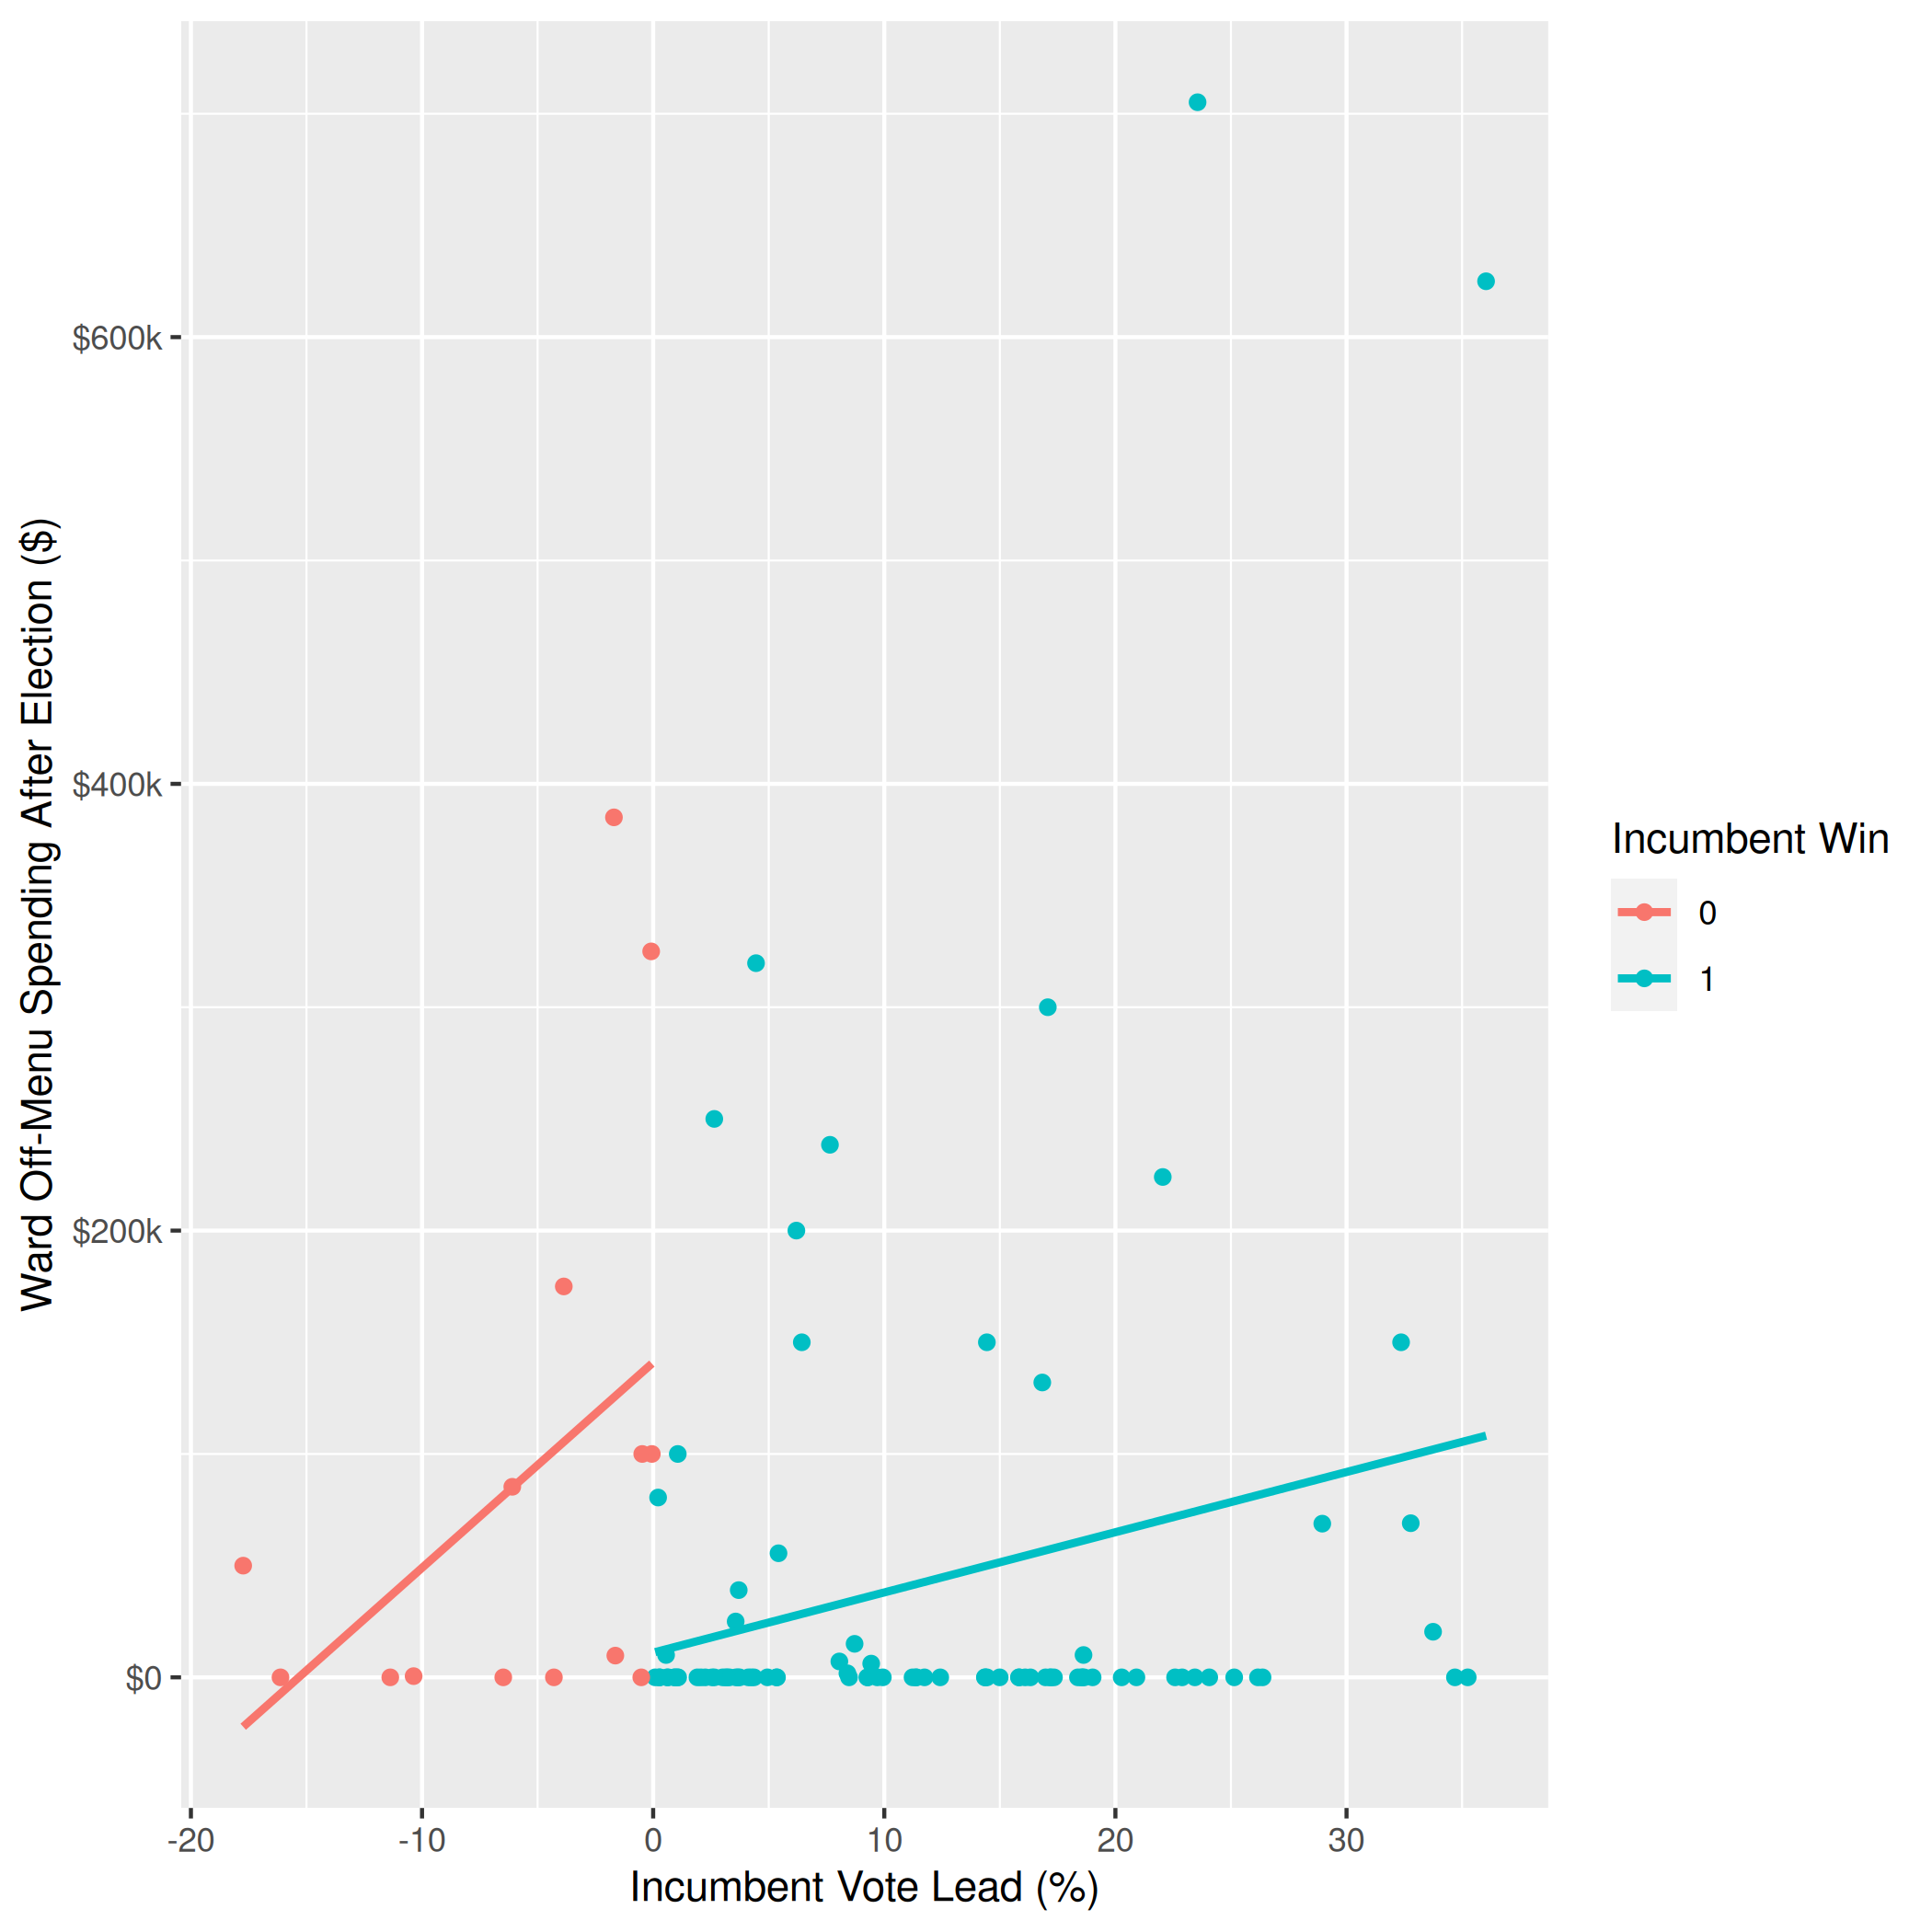
\includegraphics[scale=0.8]{input/RDD_plot.png}
        \caption{RDD results across 2011, 2015, and 2019 elections on off-menu expenditures}
\end{figure}

To verify the integrity of the regression discontinuity analysis, we perform two diagnostic procedures: A Mccrary-density test and a placebo test \cite{MCCRARY2008698}. 
The Mccrary-density test is intended to verify the random-assignment assumption, and the placebo test is intended to verify the continuity assumption. 
Starting with the Mccrary density test, we see that the visual intuition was correct. 
There is a large and statistically significant discontinuity in data density at the cutoff. 
The P-Value generated from the McCrary test is 0.00354, well below the 0.05 significance level. 
This result may be from retirement selection or the endorsement-selection reasons discussed in the methodology section. 
However, regardless of the reason for the gap, this is a significant indication that the regression discontinuity analysis is flawed.

\begin{figure}[H]
    \centering
    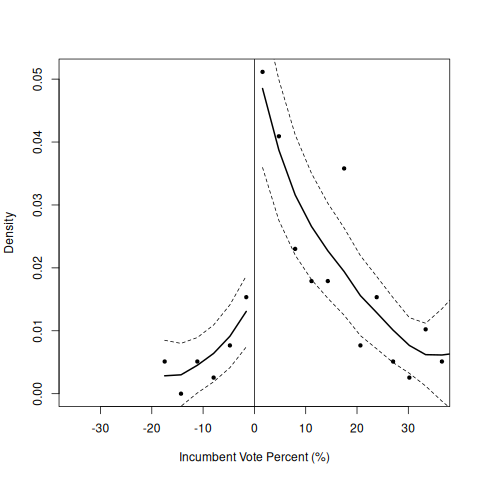
\includegraphics[scale=0.7]{input/rdd_density.png}
    \caption{Mccrary Density Test Plot}
\end{figure}

Next, we conducted a placebo test on the right side of the cutoff (due to a lack of examples of the challenger winning on the left side of the cutoff). 
We find that estimated effects range from being staunchly positive to highly negative as we move further away from the cutoff. 
However, out of 20 placebo tests, 5 achieve statistically significant levels, which is deeply concerning as it may indicate that the data generating process is inherently discontinuous, so the assumption of continuity concerning the running variable may be violated. 

\begin{figure}[H]
    \centering
    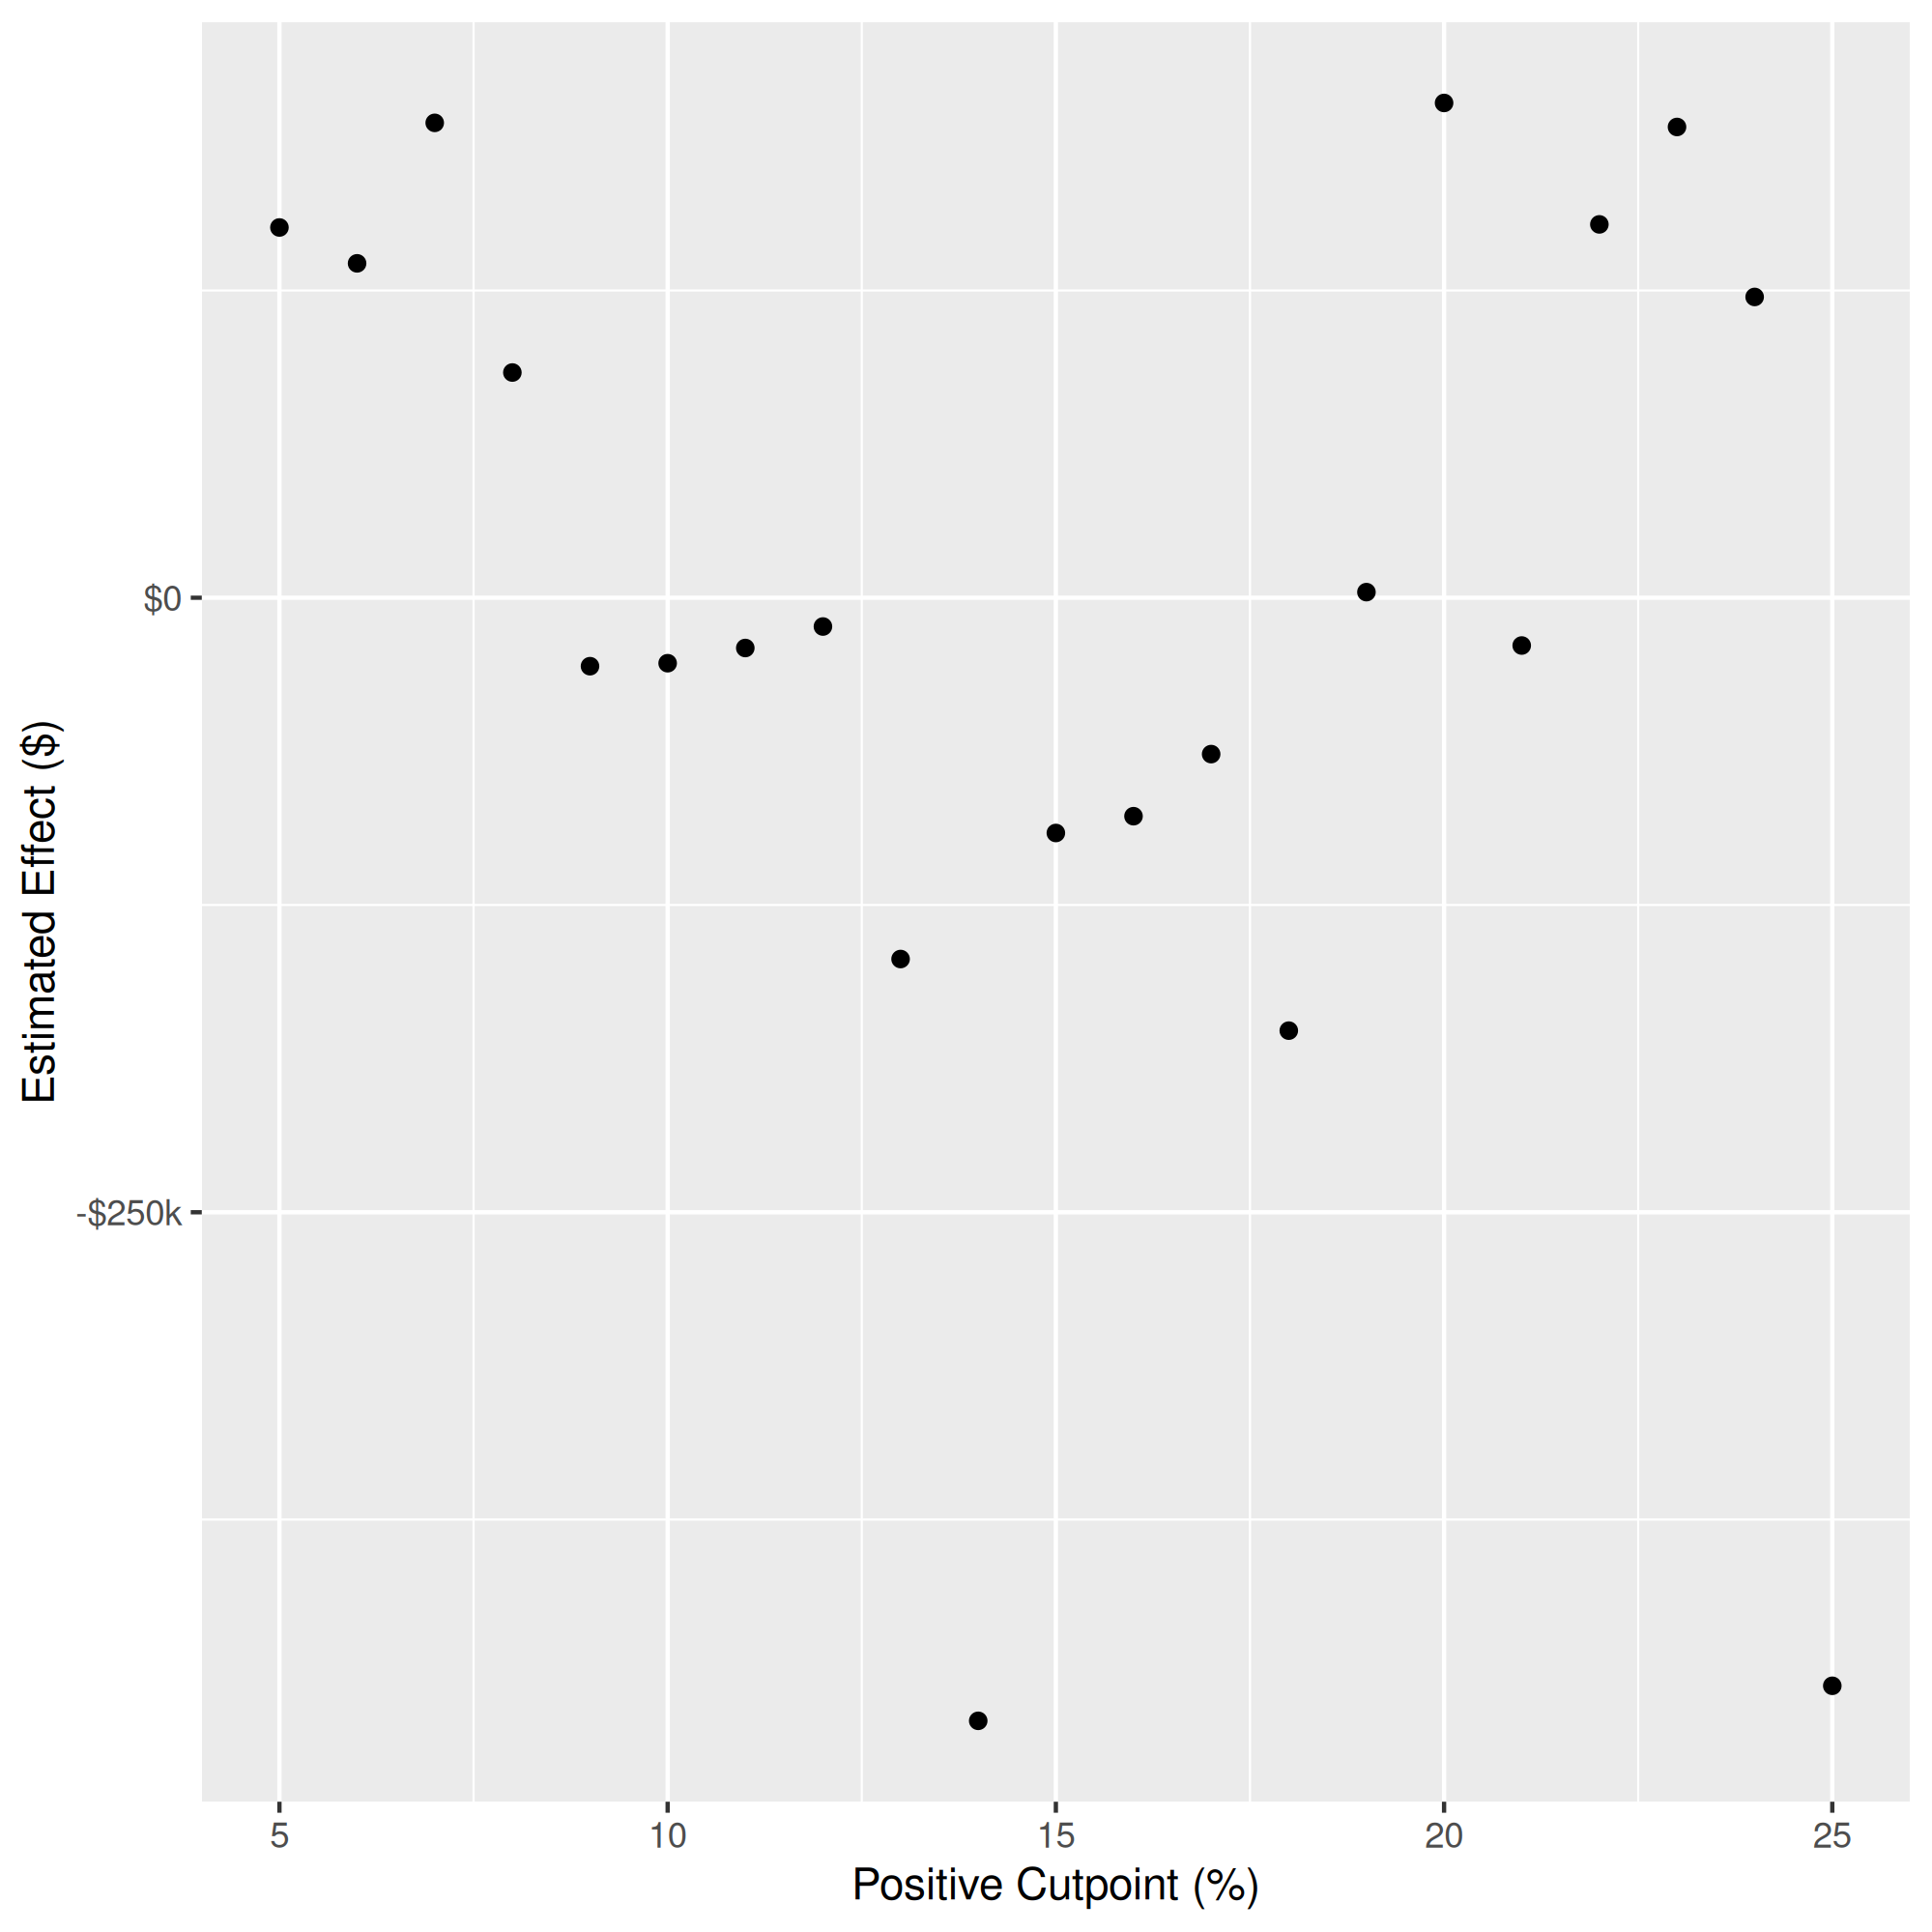
\includegraphics[scale=0.8]{input/placebo_test_effects.png}
    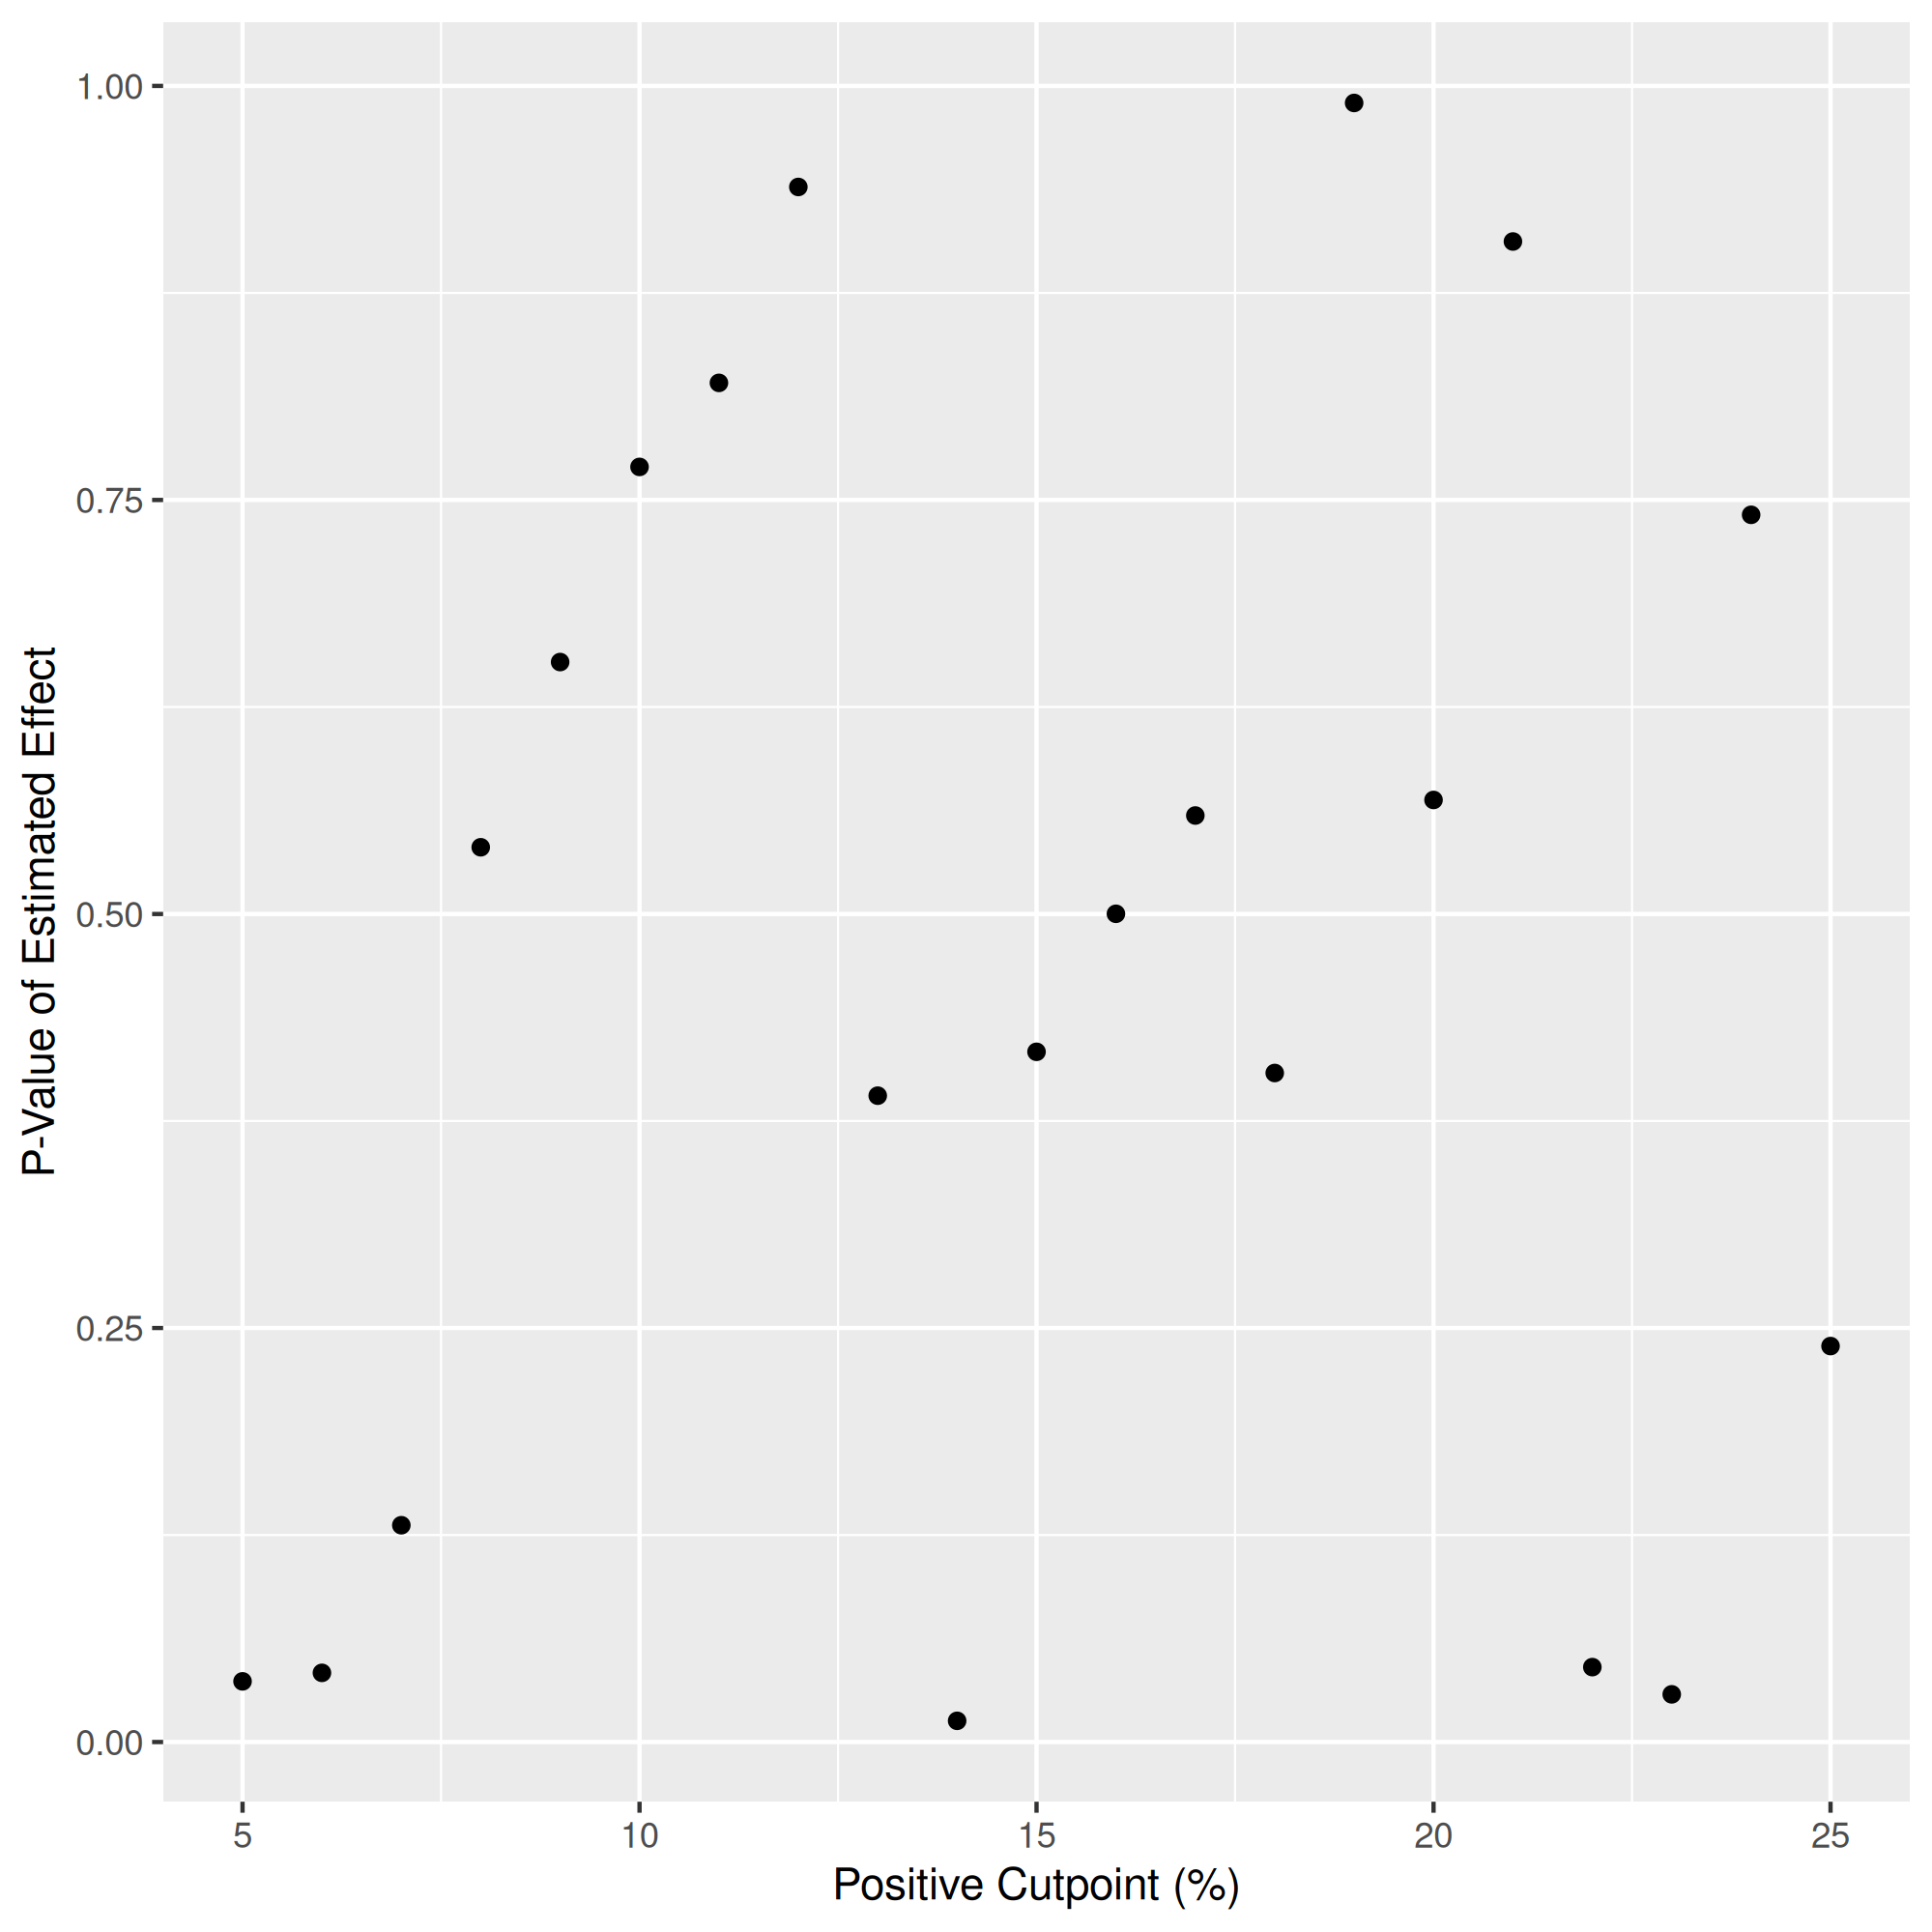
\includegraphics[scale=0.8]{input/placebo_test_pvalue.png}
    \caption{Placebo Test Results}
\end{figure}

Now moving towards diff-in-diff analysis, we show the development of the treated and non-treated wards, where treated wards are the 12 wards where the previous alderman either was elected out of the office or retired in 2015. 
From the plot, off-menu expenditures track between both groups closely prior to 2016 and then take a significant increase. 
Note that alderpersons typically take over control of the menu fund the year after they get elected \cite{particpatory_budgeting_scrapping} since they asked to approve the budget of their predecessor. 
Thus, this plot can be seen as profoundly consistent with the concept that newer alderpersons tend to spend more on off-menu expenditures. 


\begin{figure}[H]
    \centering
    \includegraphics[scale=0.8]{input/did_plot.png}
    \caption{Line plot of Off-menu expenditures}
\end{figure}

The results of the simple TWFE DiD analysis are given below in table 5. 
We include three specifications, one that uses all data and treats retiring alderpersons and council members elected out of office equally, and one reduced specification for each treatment. 
$treated_1$ is the dummy variable indicating that a group is in the post-period of 2016 on-wards and is in the treatment group. 
Each subsequent $treated$ variable estimates the effect in the post-period, so $treated_2$ is the estimate for the 2017 period, and so on. 
The 50 data points from 2020 are excluded due to the 2019 election. 

% Table created by stargazer v.5.2.3 by Marek Hlavac, Social Policy Institute. E-mail: marek.hlavac at gmail.com
% Date and time: Tue, Jun 21, 2022 - 04:53:19 PM
\begin{table}[H] \centering 
  \caption{TWFE DiD specification} 
  \label{} 
\begin{tabular}{@{\extracolsep{5pt}}lccc} 
\\[-1.8ex]\hline 
\hline \\[-1.8ex] 
 & \multicolumn{3}{c}{\textit{Dependent variable:}} \\ 
\cline{2-4} 
\\[-1.8ex] & \multicolumn{3}{c}{off menu expenditures} \\ 
\\[-1.8ex] & Both & Elected Only & Retired Only\\ 
\hline \\[-1.8ex] 
 treated\_1 & 116,597.900$^{***}$ & 98,598.880$^{**}$ & 87,257.720 \\ 
  & (37,476.320) & (48,054.550) & (54,096.760) \\ 
  & & & \\ 
 treated\_2 & 76,880.010$^{**}$ & 27,719.370 & 41,346.880 \\ 
  & (37,476.320) & (48,054.550) & (54,096.760) \\ 
  & & & \\ 
 treated\_3 & 46,261.560 & 11,758.780 & 39,047.440 \\ 
  & (37,476.320) & (48,054.550) & (54,096.760) \\ 
  & & & \\ 
 treated\_4 & 22,180.280 & $-$60,015.080 & 47,998.510 \\ 
  & (37,476.320) & (48,054.550) & (54,096.760) \\ 
  & & & \\ 
 Constant & 401,848.100$^{***}$ & 51,387.300$^{**}$ & 401,106.800$^{***}$ \\ 
  & (38,318.320) & (22,857.340) & (38,839.330) \\ 
  & & & \\ 
\hline \\[-1.8ex] 
Observations & 400 & 360 & 328 \\ 
R$^{2}$ & 0.432 & 0.029 & 0.455 \\ 
Adjusted R$^{2}$ & 0.331 & $-$0.005 & 0.354 \\ 
Residual Std. Error & 101,227.700 (df = 339) & 128,918.500 (df = 347) & 101,381.900 (df = 276) \\ 
F Statistic & 4.296$^{***}$ (df = 60; 339) & 0.849 (df = 12; 347) & 4.511$^{***}$ (df = 51; 276) \\ 
\hline 
\hline \\[-1.8ex] 
\textit{Note:}  & \multicolumn{3}{r}{$^{*}$p$<$0.1; $^{**}$p$<$0.05; $^{***}$p$<$0.01} \\ 
\end{tabular} 
\end{table} 
The ATT(g,t) analysis results are depicted below, only for the full specification, including both treatments as equal. 
When the incumbent lost control of the fund in 2016, we observed a large increase in off-menu expenditures that is barely statistically significant at a level just above \$100,000, which is similar to the results shown in the discontinuity analysis and the simple TWFE analysis above. 
Furthermore, we tested parallel pre-trends using the event study framework discussed in \cite{CALLAWAY2021200} and found that we could not reject the null hypothesis of parallel pre-trends with a p-value of 0.7754. 

\begin{figure}[H]
    \centering
    \includegraphics[scale=0.8]{input/did_treatmenteffect_plot.png}
    \caption{Treatment effect plot}
\end{figure}


However, the figure above shows that the spike is largest after the election, and then the effect dies off before the next election. This effect is not what one would expect if the DiD estimator captured an electoral effect. 
If this were an electoral effect, we would most likely see the increase in off-menu expenditures happening right before the next election in 2018. However, that is not what we see. 
Thus, this is more likely some voter-selection effect. 
We looked into the 12 candidates who made up our treatment group and the primary issues in their campaigns. 
I found articles where four candidates cited public participation and presence as key themes of their campaign \, cite{wttw. 2015} \cite{dna.2015_18} \cite{dna.2015_35} \cite{dna.2015_7}. 
Thus, from this informal evidence and the data presented, the effect is more likely from the selection or the informational mechanisms and is unlikely to be the electoral mechanism. 
\section*{Conclusions}

This paper presents a theoretical argument that politicians may shift to publicly salient "conspicuous" expenditures to "shore up" their political position. 
Specifically, we test this hypothesis in the context of Chicago's Aldermanic Menu Program, which allows local politicians to tailor infrastructure expenditures in their wards unilaterally. 
We do this by showing that these politically salient expenditures, assumed to be "off-menu" expenditures, significantly impact an incumbent's vote-share through a simple discrete choice model, where TWFE removed some endogeneity. 
That analysis showed that off-menu expenditures influence voters. 
We then show with a regression discontinuity and diff-in-diff design that wards with new politicians spend a little more than \$100,000 more on politically salient expenditures than wards that re-elect incumbents or wards where incumbents do not retire. 
This argument is not without its flaws, however. 
The regression discontinuity analysis has a clear density discontinuity, and the underlying relationship between vote-share and off-menu expenditures is not continuous. 
The density discontinuity and placebo tests, respectively, substantiate these insights. 
However, the diff-in-diff argument presented seems more credible, as by inspection of the data and by a formal event-study parallel pre-trends test showing that, at the very least, the parallel trends assumption seems to work in the pre-period. 

Overall, the thesis shows some evidence for the claim that newer alderpersons are more likely to spend on off-menu expenditures. 
However, because the increase in off-menu expenditures takes place in off-election periods, it is unlikely that this is due to deliberate conspicuous expenditures for political advantage. 
In particular, if electoral motives induced this, then the result of the diff-in-diff that the primary effect on expenditures is in the period furthest away from the next election seems puzzling. 
Thus, the results of the diff-in-diff, if they provide evidence of anything, provide evidence more towards that of an experiential mechanism where alderpersons rely on public knowledge to allocate resources until they learn how to allocate it themselves or a selection mechanism where voters elect politicians most likely to listen to their input, which favors immediate interests. 
Furthermore, note that the evidence for any effect is weak at best due to the relatively high standard errors. 
More data is necessary to make more substantive conclusions on the nature of these expenditures, as it would ameliorate the estimation concerns with the diff-in-diff and allow a more precise estimation of the regression discontinuity analysis.

% -----------------------------------------------
% 	REFERENCES
% -----------------------------------------------

\bibliography{../bib/bib.bib}{}

\newpage
\clearpage

\begin{center} \Large \textbf{Appendix -- For Online Publication} \end{center}
\appendix
\numberwithin{equation}{section}
\numberwithin{figure}{section}
\numberwithin{table}{section}

\section*{Appendix: Regression Results with Beautification}

\begin{table}[H] \centering 
  \caption{Discrete Choice and TWFE results with Beautification} 
  \label{} 
\begin{tabular}{lccc} 
\\[-1.8ex]\hline 
\hline \\[-1.8ex] 
 & \multicolumn{3}{c}{\textit{Model:}} \\ 
\cline{2-4} 
\\[-1.8ex] & Discrete Choice & OLS & Experience OLS \\ 
\\[-1.8ex] & (1) & (2) & (3)\\ 
\hline \\[-1.8ex] 
 beauty & 0.281$^{**}$ & 6.690$^{**}$ & 5.696$^{*}$ \\ 
  & (0.119) & (2.770) & (2.833) \\ 
  & & & \\ 
 exp &  &  & $-$0.447 \\ 
  &  &  & (0.343) \\ 
  & & & \\ 
 Constant & $-$0.941$^{*}$ & 27.667$^{**}$ & 33.379$^{**}$ \\ 
  & (0.532) & (12.345) & (12.928) \\ 
  & & & \\ 
\hline \\[-1.8ex] 
Observations & 71 & 71 & 71 \\ 
R$^{2}$ & 0.863 & 0.846 & 0.857 \\ 
Adjusted R$^{2}$ & 0.583 & 0.532 & 0.546 \\ 
Residual Std. Error & 0.329 (df = 23) & 7.643 (df = 23) & 7.530 (df = 22) \\ 
F Statistic & 3.078$^{***}$ (df = 47; 23) & 2.696$^{***}$ (df = 47; 23) & 2.755$^{***}$ (df = 48; 22) \\ 
\hline 
\hline \\[-1.8ex] 
\textit{Note:}  & \multicolumn{3}{r}{$^{*}$p$<$0.1; $^{**}$p$<$0.05; $^{***}$p$<$0.01} \\ 
\end{tabular} 
\end{table} 


\begin{table}[H] \centering 
  \caption{OLS Results with Unopposed Candidates Included} 
  \label{} 
\begin{tabular}{@{\extracolsep{5pt}}lcc} 
\\[-1.8ex]\hline 
\hline \\[-1.8ex] 
 & \multicolumn{2}{c}{\textit{Dependent variable:}} \\ 
\cline{2-3} 
\\[-1.8ex] & \multicolumn{2}{c}{Vote Share} \\ 
\\[-1.8ex] & (1) & (2)\\ 
\hline \\[-1.8ex] 
 off\_menu & 4.918 &  \\ 
  & (3.654) &  \\ 
  & & \\ 
 exp &  & $-$0.949 \\ 
  &  & (0.626) \\ 
  & & \\ 
 Constant & 32.639 & 55.827$^{***}$ \\ 
  & (20.171) & (15.028) \\ 
  & & \\ 
\hline \\[-1.8ex] 
Observations & 83 & 83 \\ 
R$^{2}$ & 0.727 & 0.731 \\ 
Adjusted R$^{2}$ & 0.301 & 0.311 \\ 
Residual Std. Error (df = 32) & 14.804 & 14.699 \\ 
F Statistic (df = 50; 32) & 1.705$^{*}$ & 1.739$^{**}$ \\ 
\hline 
\hline \\[-1.8ex] 
\textit{Note:}  & \multicolumn{2}{r}{$^{*}$p$<$0.1; $^{**}$p$<$0.05; $^{***}$p$<$0.01} \\ 
\end{tabular} 
\end{table} 



% Table created by stargazer v.5.2.3 by Marek Hlavac, Social Policy Institute. E-mail: marek.hlavac at gmail.com
% Date and time: Tue, Jan 24, 2023 - 08:33:57 PM
\begin{table}[H] \centering 
  \caption{Regression Discontinuity Results with Beautification} 
  \label{rdd_cutoff_table_beauty} 
\small 
\begin{tabular}{@{\extracolsep{0pt}}lcccc} 
\\[-1.8ex]\hline 
\hline \\[-1.8ex] 
 & \multicolumn{4}{c}{Bandwidth Criterion:} \\ 
\cline{2-5} 
\\[-1.8ex] & \multicolumn{4}{c}{beauty} \\ 
 & Full & IK & MSE & CER \\ 
\\[-1.8ex] & (1) & (2) & (3) & (4)\\ 
\hline \\[-1.8ex] 
 IW & 397 & 251 & 253 & 524 \\ 
  & (6,577) & (6,874) & (8,428) & (9,127) \\ 
  & & & & \\ 
 IVS & $-$2,016 & $-$2,016 & $-$7,480 & $-$37,940 \\ 
  & (75,033) & (75,044) & (237,448) & (342,903) \\ 
  & & & & \\ 
 IW:IVS & 1,930 & 3,542 & 11,355 & 44,949 \\ 
  & (75,725) & (79,608) & (243,401) & (354,017) \\ 
  & & & & \\ 
 Constant & 49,575$^{***}$ & 49,575$^{***}$ & 49,450$^{***}$ & 49,090$^{***}$ \\ 
  & (6,077) & (6,078) & (7,567) & (8,113) \\ 
  & & & & \\ 
\hline \\[-1.8ex] 
Observations & 4,150 & 3,250 & 2,300 & 1,900 \\ 
R$^{2}$ & 0 & 0 & 0 & 0 \\ 
Adjusted R$^{2}$ & $-$0 & $-$0 & $-$0 & $-$0 \\ 
Residual Std. Error & 103,521 (df = 4146) & 103,536 (df = 3246) & 103,532 (df = 2296) & 103,546 (df = 1896) \\ 
F Statistic & 0 (df = 3; 4146) & 0 (df = 3; 3246) & 0 (df = 3; 2296) & 0 (df = 3; 1896) \\ 
\hline 
\hline \\[-1.8ex] 
\textit{Note:}  & \multicolumn{4}{r}{$^{*}$p$<$0.1; $^{**}$p$<$0.05; $^{***}$p$<$0.01} \\ 
\end{tabular} 
\end{table} 


% Table created by stargazer v.5.2.3 by Marek Hlavac, Social Policy Institute. E-mail: marek.hlavac at gmail.com
% Date and time: Sun, Jul 17, 2022 - 03:52:33 PM
\begin{table}[H] \centering 
  \caption{Diff-in-Diff Results with Beautification} 
  \label{} 
\begin{tabular}{@{\extracolsep{5pt}}lccc} 
\\[-1.8ex]\hline 
\hline \\[-1.8ex] 
 & \multicolumn{3}{c}{\textit{Treatment Variable:}} \\ 
\cline{2-4} 
\\
\\[-1.8ex] & Both & Electoral Only & Retirement Only\\ 
\hline \\[-1.8ex] 
 treated & 96,202.610$^{***}$ & 105,220.300$^{**}$ & 81,802.030$^{*}$ \\ 
  & (33,413.550) & (41,793.240) & (47,734.510) \\ 
  & & & \\ 
 treated\_1 & $-$50,774.430 & $-$99,109.770$^{*}$ & $-$44,385.510 \\ 
  & (42,265.170) & (59,103.990) & (60,379.910) \\ 
  & & & \\ 
 treated\_2 & 8,470.087 & 33,825.860 & 17,229.070 \\ 
  & (42,265.170) & (59,103.990) & (60,379.910) \\ 
  & & & \\ 
 treated\_3 & $-$30,194.430 & $-$82,640.400 & 1,600.154 \\ 
  & (42,265.170) & (59,103.990) & (60,379.910) \\ 
  & & & \\ 
 treated\_4 & 27,918.280 & 27,503.180 & 36,145.330 \\ 
  & (42,265.170) & (59,103.990) & (60,379.910) \\ 
  & & & \\ 
 Constant & 297,785.700$^{***}$ & 56,001.950$^{***}$ & 298,376.600$^{***}$ \\ 
  & (32,512.140) & (18,688.580) & (32,644.510) \\ 
  & & & \\ 
\hline \\[-1.8ex] 
Observations & 450 & 405 & 378 \\ 
R$^{2}$ & 0.355 & 0.050 & 0.382 \\ 
Adjusted R$^{2}$ & 0.252 & 0.016 & 0.279 \\ 
Residual Std. Error & 90,253.700 (df = 387) & 107,186.800 (df = 390) & 89,606.330 (df = 323) \\ 
F Statistic & 3.440$^{***}$ (df = 62; 387) & 1.466 (df = 14; 390) & 3.696$^{***}$ (df = 54; 323) \\ 
\hline 
\hline \\[-1.8ex] 
\textit{Note:}  & \multicolumn{3}{r}{$^{*}$p$<$0.1; $^{**}$p$<$0.05; $^{***}$p$<$0.01} \\ 
\end{tabular} 
\end{table} 
%\input{./sections/appendix_data.tex}
%\input{./sections/appendix_empirics.tex}

\end{document}